\section{Külső szolgáltatások és függőségek}

A WatchDB nem teljesen önálló rendszerként működik, hanem több külső szolgáltatásra és fejlesztői csomagra épül. Ezek a függőségek gyorsítják a fejlesztést, mert nem szükséges saját teljes filmadatbázist vagy egyedi UI komponenseket kialakítani. Ugyanakkor a választott szolgáltatások elérhetősége, verziói és használati feltételei közvetlenül hatnak az alkalmazás működésére.

A legfontosabb külső szolgáltatások és függőségek a következők:

\begin{itemize}
    \item \textbf{Supabase}: a felhasználóhoz kötött adatok tárolását biztosítja. A projektben a \texttt{watchlist} és \texttt{watched} táblák kapcsolódnak hozzá. Szolgáltatáskimaradás vagy hibás konfiguráció esetén a személyes funkciók nem érhetők el.
    \item \textbf{TMDB API}: külső filmadatforrásként működik. A filmkeresés, a filmrészletek, a poszterek és háttérképek lekérése ezen keresztül történik \cite{tmdbApiGettingStarted}. API-korlát, lassulás vagy elérhetetlenség esetén a keresés és a filmoldalak működésének minősége gyengülhet.
    \item \textbf{Vercel / Next.js környezet}: az alkalmazás futtatását, az oldalak kiszolgálását és a szerveroldali route-ok kezelését támogatja. Build- vagy deployment-hiba esetén az új verzió nem kerül élesítésre.
    \item \textbf{TanStack Query}: a kliensoldali szerverállapot-kezelésért felel. A watchlist és watched állapotok lekérése, a mutációk (\texttt{CREATE, UPDATE, DELETE}) kezelése és a cache-frissítés is ehhez kapcsolódik. Hibás invalidálás esetén a felület ideiglenesen elavult adatot mutathat, bár ez a hiba inkább fejlesztői oldalról történhet meg, nem pedig egy külső szolgáltatástól függ.
    \item \textbf{UI függőségek}: a felületi komponensek és stílusok kialakítását segítik. Ide tartozik a Tailwind CSS, a Radix UI, a shadcn/ui jellegű komponensek és az ikonok. Verzióváltáskor megjelenési vagy komponens-kompatibilitási problémák jelentkezhetnek.
\end{itemize}

A felsorolt külső szolgáltatások és a velük járó kockázatok mind számításba lettek véve a fejlesztési folyamatot megelőző tervezési szakaszban.

A külső filmadatok eléréséhez a projekt a \texttt{TMDB\_ACCESS\_TOKEN} környezeti változót használja. Ez csak szerveroldalon kerül felhasználásra, ezért a böngésző közvetlenül nem kap hozzáférést a tokenhez. Ez a döntés biztonsági szempontból fontos, mert így a külső API-hoz tartozó hozzáférési adat nem jelenik meg a kliensoldali kódban.

A fejlesztői csomagok szintén fontos függőséget jelentenek. A \texttt{package.json} alapján a projekt fő futásidejű csomagjai közé tartozik a \texttt{next}, a \texttt{react}, a \texttt{@supabase/ssr}, a \texttt{@supabase/supabase-js}, a \texttt{@tanstack/react-query}, valamint a felülethez kapcsolódó Radix UI, Tailwind és ikoncsomagok. Ezek verzióit kontrolláltan kell frissíteni, mert egy nagyobb keretrendszer- vagy könyvtárfrissítés érintheti az útvonalkezelést, a szerveroldali működést, az adatkapcsolatot vagy a komponensek viselkedését, esetleges biztonsági patcheket is tartalmazhatnak az új verziók.

\begin{figure}[H]
    \centering
    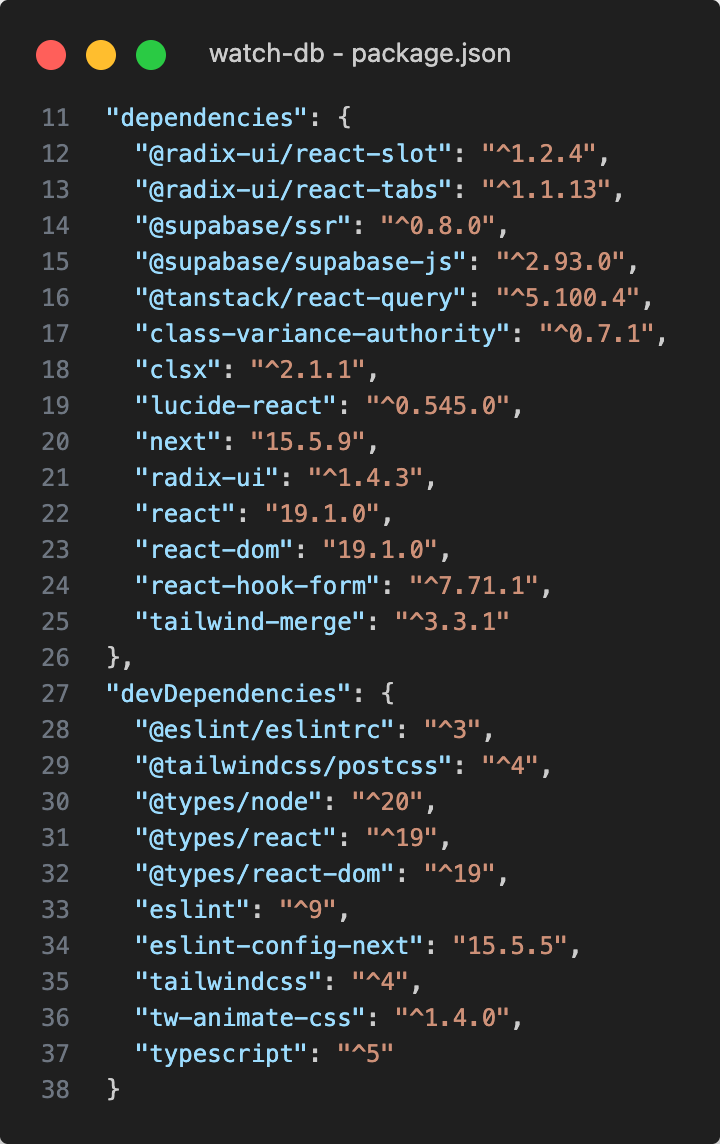
\includegraphics[height=0.68\textheight]{chapters/chapter-5-systemSpecs/dependencies.png}
    \caption{A projekt fő függőségei a \texttt{package.json} alapján}
    \label{fig:watchdb-dependencies}
\end{figure}

A külső függőségek kezelése miatt a projekt elkülöníti a szolgáltatásrétegeket. A TMDB-vel kommunikáló kód külön modulba került. A Supabase kliens inicializálása külön böngészőoldali és szerveroldali fájlban szerepel. Ez a szervezés csökkenti annak kockázatát, hogy egy külső szolgáltatáshoz kapcsolódó változás az alkalmazás több, egymástól távoli részét érintse.
